\section{Differential Calculus}

\begin{Theorem}{
    Fundamental Lemma\footnote{\href{https://trello.com/c/byu9Pyy8}{Calculus with Analytic Geometry by George F. Simmons}, p. 680}
    \phantomsection\hypertarget{fundamental-lemma}
}{fundamental-lemma}
    Suppose that a function $z = f(x, y)$ and its partial derivatives $f_x$ and $f_y$ are defined at a point
    $(x_0, y_0)$, and also through some neighborhood of this point. Suppose further that $f_x$ and $f_y$ are continuous
    at $(x_0, y_0)$. Then the increment $\Delta z$ can be expressed in the form of

    \begin{equation}
        \Delta z = f_x(x_0, y_0)\Delta x + f_y(x_0, y_0)\Delta y + \epsilon_1\Delta x + \epsilon_2\Delta y
    \end{equation}

    where $\epsilon_1$ and $\epsilon_2 \rightarrow 0$ as $\Delta x$ and $\Delta y \rightarrow 0$
\end{Theorem}

To prove this
statement\footnote{\href{https://trello.com/c/byu9Pyy8}{Calculus with Analytic Geometry by George F. Simmons}, p. 841},
we analyze the change $\Delta z$ in 2 steps as shown in Fig.~\ref{fig:proof-fundamental-lemma}:

\begin{figure}[H]
    \centering
    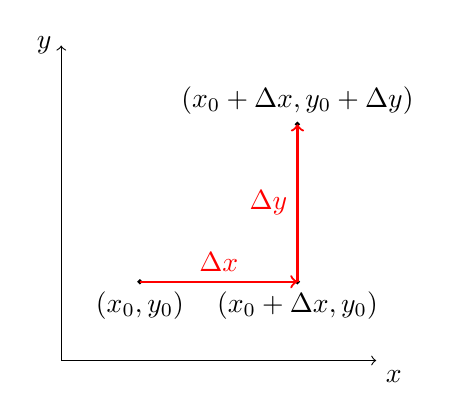
\begin{tikzpicture}
        \draw [<->] (0,4) -- (0,0) -- (4,0);
        \node [below right] at (4,0) {$x$};
        \node [left] at (0,4) {$y$};

        \draw[fill] (1,1) circle [radius=0.025];
        \draw[fill] (3,1) circle [radius=0.025];
        \draw[fill] (3,3) circle [radius=0.025];

        \node [below] at (1,1) {$(x_0, y_0)$};
        \node [below] at (3,1) {$(x_0 + \Delta x, y_0)$};
        \node [above] at (3,3) {$(x_0 + \Delta x, y_0 + \Delta y)$};

        \draw [->][thick, red] (1,1) -- node[above] {$\Delta x$} (3,1);
        \draw [->][thick, red] (3,1) -- node[left] {$\Delta y$} (3,3);
    \end{tikzpicture}
    \caption{We assume $\Delta z = f(x_0 + \Delta x, y_0 + \Delta y) - f(x_0, y_0)$ and $\Delta z = \Delta_1 z + \Delta_2 z$}
    \label{fig:proof-fundamental-lemma}
\end{figure}

\begin{enumerate}
    \item changing $x$ alone and moving from $(x_0, y_0)$ to $(x_0 + \Delta x, y_0)$, and then
    \item changing $y$ alone and moving from $(x_0 + \Delta x, y_0)$ to $(x_0 + \Delta x, y_0 + \Delta y)$
\end{enumerate}

We denote the first change in $z$ by $\Delta_1 z$, so that

\begin{equation}
    \Delta_1 z = f(x_0 + \Delta x, y_0) - f(x_0, y_0)
\end{equation}

By The Mean Value Theorem\footnote{
    \begin{Theorem}{
        The Mean Value Theorem\footnote{\href{https://trello.com/c/byu9Pyy8}{Calculus with Analytic Geometry by George F. Simmons}, p. 76}
    }{mean-value-theorem}
        Let $y = f(x)$ be a function with the following two properties:

        \begin{enumerate}
            \item $f(x)$ is continuous on the closed interval $[a, b]$; and
            \item $f(x)$ is differentiable on the open interval $(a, b)$
        \end{enumerate}

        Then there exists at least one point $c$ in the open interval $(a, b)$ such that

        \[
            f'(c) = \frac{f(b) - f(a)}{b - a}
        \]

        or equivalently,

        \[
            f(b) - f(a) = f'(c)(b - a)
        \]
    \end{Theorem}
}, we can write this as

\begin{equation}\label{eq:first-change-z-mean-val-theo}
\Delta_1 z = \Delta x f_x(x_1, y_0)
\end{equation}

where $x_1$ is between $x_0$ and $x_0 + \Delta x$. Smilary, if we denote the second part of the change in $z$ by
$\Delta_1 z$, so that

\begin{equation}
    \Delta_2 z = f(x_0 + \Delta x, y_0 + \Delta y) - f(x_0 + \Delta x, y_0)
\end{equation}

then

\begin{equation}\label{eq:second-change-z-mean-val-theo}
\Delta_2 z = \Delta y f_y(x_0 + \Delta x, y_1)
\end{equation}

where $y_1$ is between $y_0$ and $y_0 + \Delta y$.

Now as $\Delta x$ and $\Delta y \rightarrow 0$, $x_1 \rightarrow x_0$ and $y_1 \rightarrow y_0$. By the assumed
continuity of $f_x$ and $f_y$ at $(x_0, y_0)$, we can write

\begin{align}
    f_x(x_1, y_0) = f_x(x_0, y_0) + \epsilon_1 \label{eq:first-change-z-epsilon} \\
    f_y(x_0 + \Delta x, y_1) = f_y(x_0, y_0) + \epsilon_2 \label{eq:second-change-z-epsilon}
\end{align}

where $\epsilon_1$ and $\epsilon_2 \rightarrow 0$ as $\Delta x$ and $\Delta y \rightarrow 0$. Plugging
Eq.\ref{eq:first-change-z-epsilon} into Eq.\ref{eq:first-change-z-mean-val-theo} gives us

\begin{equation}
    \Delta_1 z = \Delta x\left[ f_x(x_0, y_0) + \epsilon_1 \right] = \Delta x f_x(x_0, y_0) + \Delta x\epsilon_1
\end{equation}

and similarly Eq.\ref{eq:second-change-z-epsilon} into Eq.\ref{eq:second-change-z-mean-val-theo}

\begin{equation}
    \Delta_2 z = \Delta y\left[ f_y(x_0, y_0) + \epsilon_2 \right] = \Delta y f_y(x_0, y_0) + \Delta y\epsilon_2
\end{equation}

Since we have assumed $\Delta z = \Delta_1 z + \Delta_2 z$

\begin{equation}
    \Delta z = \Delta x f_x(x_0, y_0) + \Delta x\epsilon_1 + \Delta y f_y(x_0, y_0) + \Delta y\epsilon_2 = f_x(x_0, y_0)\Delta x + f_y(x_0, y_0)\Delta y + \epsilon_1\Delta x + \epsilon_2\Delta y
\end{equation}

\qed

\footnote{\href{https://trello.com/c/byu9Pyy8}{Calculus with Analytic Geometry by George F. Simmons}, p. 681} Now Let
$f(x, y, z)$ be a function of 3 variables defined throughout some region of three-dimensional space, and let $P$ be a
point in this region. At what rate does $f$ change as we move away from $P$ in a specified direction? In the directions
of the positive x, y, and z-axes, we know that the rates of change off are given by the partial derivatives
$\frac{\partial f}{\partial x}$, $\frac{\partial f}{\partial y}$, and $\frac{\partial f}{\partial z}$. But how do we
calculate the rate of change of $f$ if we move away from $P$ in a direction that is not a coordinate direction?

Let $P = (x, y, z)$ and $\boldsymbol{R} = x\boldsymbol{i} + y\boldsymbol{j} + z\boldsymbol{k}$ being the position vector
of $P$. If we move away from $P$ to a nearby point $Q = (x + \Delta x, y + \Delta y, z + \Delta z)$, then the function
will change by an amoutn $\Delta f$. Let $\Delta s$ denote the distance between $P$ and $Q$, then we have

\begin{equation}\label{eq:def-df-over-ds}
    \frac{df}{ds} = \lim\limits_{\Delta s \rightarrow 0}\frac{\Delta f}{\Delta s}
\end{equation}

We further assume that $f(x, y, z)$ has continuous partial derivatives with respect to $x$, $y$, and $z$.

\begin{marker}
    Unless explicitly stated otherwise, all functions we deal with are always continuous in all of our discussions
\end{marker}

The \hyperlink{fundamental-lemma}{Fundamental Lemma} enables us to write $\Delta f$ in the form of

\begin{equation}\label{eq:df-in-3-partials}
    \Delta f = \frac{\partial f}{\partial x}\Delta x + \frac{\partial f}{\partial y}\Delta y + \frac{\partial f}{\partial z}\Delta z + \epsilon_1\Delta x + \epsilon_2\Delta y + \epsilon_3\Delta z
\end{equation}

As $\Delta s \rightarrow 0$, i.e. as $\Delta x \rightarrow 0$, $\Delta y \rightarrow 0$, and $\Delta z \rightarrow 0$,
$\epsilon_1, \epsilon_2, \epsilon_3 \rightarrow 0$. Dividing Eq.\ref{eq:df-in-3-partials} by $\Delta s$ gives

\begin{equation}\label{eq:df-over-ds-in-3-partials}
    \lim\limits_{\Delta s \rightarrow 0}\frac{\Delta f}{\Delta s} = \frac{\partial f}{\partial x}\frac{dx}{ds} + \frac{\partial f}{\partial y}\frac{dy}{ds} + \frac{\partial f}{\partial z}\frac{dz}{ds}
\end{equation}

Combing Eq.\ref{eq:df-over-ds-in-3-partials} and \ref{eq:def-df-over-ds} results in

\begin{equation}\label{eq:partial-chain-rule}
    \tcbhighmath[
        enhanced,colframe=red,colback=white,arc=0pt,boxrule=1pt,
        fuzzy halo=1mm with blue!50!white,
        arc=2pt,
        boxrule=0pt,
        frame hidden
    ]{
        \frac{df}{ds} = \frac{\partial f}{\partial x}\frac{dx}{ds} + \frac{\partial f}{\partial y}\frac{dy}{ds} + \frac{\partial f}{\partial z}\frac{dz}{ds}
    }
\end{equation}

\subsection{Gradient}



\begin{equation}
    dT = \left( \frac{\partial T}{\partial x} \right) dx + \left( \frac{\partial T}{\partial y} \right) dy + \left( \frac{\partial T}{\partial z} \right) dz
\end{equation}